\documentclass[border=6pt]{standalone}
\usepackage{tikz}
\usetikzlibrary{arrows.meta,positioning,calc}
\begin{document}
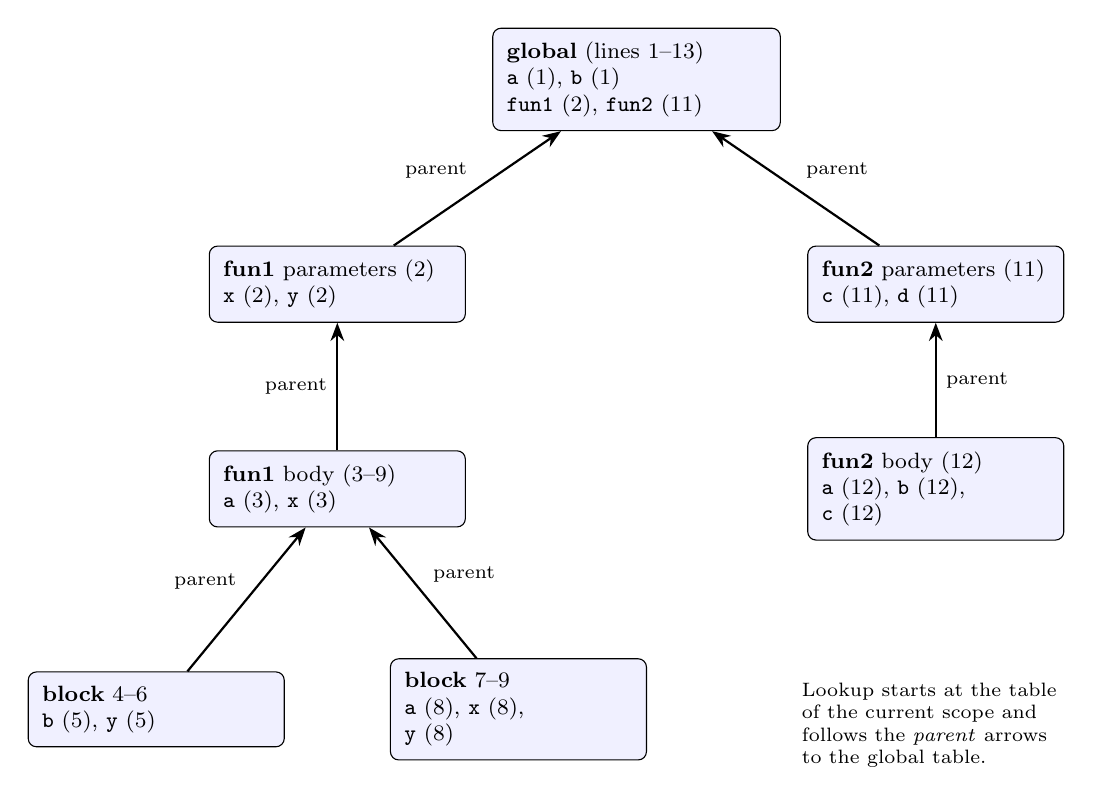
\begin{tikzpicture}[>=Stealth,font=\small,
  tbl/.style={draw,rounded corners=3pt,fill=blue!6,align=left,inner sep=5pt,font=\footnotesize,text width=2.9cm},
  hd/.style={font=\footnotesize\bfseries}]
\node[tbl,text width=3.3cm] (G) at (3.8,0) {\textbf{global} (lines 1--13)\\ \texttt{a}\ (1), \texttt{b}\ (1)\\ \texttt{fun1}\ (2), \texttt{fun2}\ (11)};
\node[tbl] (F1p) at (0,-2.6) {\textbf{fun1} parameters (2)\\ \texttt{x}\ (2), \texttt{y}\ (2)};
\node[tbl] (F2p) at (7.6,-2.6) {\textbf{fun2} parameters (11)\\ \texttt{c}\ (11), \texttt{d}\ (11)};
\node[tbl] (F1b) at (0,-5.2) {\textbf{fun1} body (3--9)\\ \texttt{a}\ (3), \texttt{x}\ (3)};
\node[tbl] (F2b) at (7.6,-5.2) {\textbf{fun2} body (12)\\ \texttt{a}\ (12), \texttt{b}\ (12),\\ \texttt{c}\ (12)};
\node[tbl] (B1) at (-2.3,-8) {\textbf{block} 4--6\\ \texttt{b}\ (5), \texttt{y}\ (5)};
\node[tbl] (B2) at (2.3,-8) {\textbf{block} 7--9\\ \texttt{a}\ (8), \texttt{x}\ (8),\\ \texttt{y}\ (8)};
\draw[->,thick] (F1p) -- node[above left,font=\scriptsize]{parent} (G);
\draw[->,thick] (F2p) -- node[above right,font=\scriptsize]{parent} (G);
\draw[->,thick] (F1b) -- node[left,font=\scriptsize]{parent} (F1p);
\draw[->,thick] (F2b) -- node[right,font=\scriptsize]{parent} (F2p);
\draw[->,thick] (B1) -- node[above left,font=\scriptsize]{parent} (F1b);
\draw[->,thick] (B2) -- node[above right,font=\scriptsize]{parent} (F1b);
% stack of "current scope" pointer examples
\node[font=\scriptsize,align=left,text width=3.4cm] at (7.6,-8.2) {Lookup starts at the table of the current scope and follows the \emph{parent} arrows to the global table.};
\end{tikzpicture}
\end{document}
